\documentclass{beamer}
\usepackage[latin1]{inputenc}
\usetheme{Warsaw}
\title{Introducci�n a Flask}
\subtitle{No lo hagas complicado si puede ser simple}
\begin{document}

\begin{frame}
\titlepage
\end{frame}

\begin{frame}

\includegraphics[width=\textwidth]{imagenes/wth.jpg}
\end{frame}

\begin{frame}{Historia y origen}
\begin{itemize}
\item Es un microframework para desarrollo web en Python
\item Se basa en dos pilares: Werkzeug (WSGI), Jinja2 (plantillas)
\item Es software libre (desarrollo en github)
\end{itemize}
\end{frame}

\begin{frame}{�Para qu� es bueno Flask IMHO?}

Es bueno para:
\begin{itemize}
\item Prototipado r�pido
\item Requisitos hardware muy estrictos (Raspberry Pi)
\item Encaja en la filosof�a de micro servicios
\end{itemize}

\vspace{1cm}

NO es bueno para:
\begin{itemize}
\item Reemplazo de Django
\item Un proyecto de gran envergadura
\end{itemize}
\end{frame}

\begin{frame}{Filosof�a}
\begin{itemize}
\item Mantener el n�cleo simple pero f�cilmente extensible
\item Convenci�n sobre configuraci�n
\item Muy buena y ordenada documentaci�n
\end{itemize}
\end{frame}

\begin{frame}{Ejemplo b�sico}
\begin{center}

\includegraphics[width=0.7\textwidth]{imagenes/code.jpg}
\end{center}
\end{frame}

\begin{frame}{Virtualenv}
\begin{center}
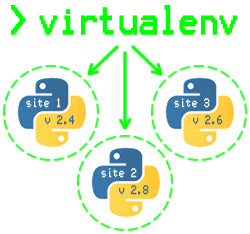
\includegraphics[width=0.6\textwidth]{imagenes/virtualenv.jpg}
\end{center}
\end{frame}

\begin{frame}{}
\begin{center}

\includegraphics[width=0.7\textwidth]{imagenes/impossibru.jpg}
\end{center}
\end{frame}

\begin{frame}{Extensiones de Flask}
\begin{itemize}
\item Flask-Admin
\item Flask-Cache
\item Flask-SQLAlchemy
\item Flask-WTF
\item Flask-Mail
\item Flask-MongoAlchemy
\item Flask-OpendID
\end{itemize}
\end{frame}

\begin{frame}{Ejemplo pr�ctico: Raspberry Pi}

\includegraphics[width=\textwidth]{imagenes/chuck.jpg}
\end{frame}

\begin{frame}{Recursos}
\begin{itemize}
\item Esta presentaci�n y ejemplos: https://github.com/mzaforas/seminario-flask
\item Documentaci�n oficial: http://flask.pocoo.org/docs/
\item Extensiones: http://flask.pocoo.org/extensions/
\end{itemize}
\end{frame}

\begin{frame}
\begin{center}

\includegraphics[width=0.6\textwidth]{imagenes/questions.jpg}
\end{center}

\end{frame}

\end{document}
